\documentclass[conference]{IEEEtran}
\IEEEoverridecommandlockouts
% The preceding line is only needed to identify funding in the first footnote. If that is unneeded, please comment it out.
\usepackage{cite}
\usepackage{amsmath,amssymb,amsfonts}
\usepackage{algorithmic}
\usepackage{graphicx}
\usepackage{textcomp}
\usepackage{xcolor}
\usepackage{float}
\def\BibTeX{{\rm B\kern-.05em{\sc i\kern-.025em b}\kern-.08em
    T\kern-.1667em\lower.7ex\hbox{E}\kern-.125emX}}
\begin{document}

\title{Analisi esplorativa del tasso di suicidio annuale in diversi paesi su dataset WHO\\
{\footnotesize Tesina di Data Science for Health Systems}
}

\author{\IEEEauthorblockN{Paolo Speziali}
\IEEEauthorblockA{\textit{Dipartimento di Ingegneria} \\
\textit{Università degli Studi di Perugia}\\
Perugia, Italia \\
paolo.speziali@studenti.unipg.it}
}

\maketitle

\begin{abstract}
Questo documento riporta i risultati dell'analisi esplorativa del dataset fornito dalla
World Health Organization relativo al tasso di mortalità per suicidio standardizzato per età.
L'obiettivo di questa analisi è quello di esaminare se, in differenti paesi nel corso degli anni,
la distribuzione annuale del tasso di suicidi sia significativamente differente o meno,
aprendo la strada a potenziali
ipotesi su fenomeni globali che possono averne influenzato la tendenza.
Tramite l'analisi di quattro gruppi di soggetti è possibile osservare come una
distribuzione senza differenze significative emerga solo in pochi casi.
\end{abstract}

\begin{IEEEkeywords}
suicide, EDA, WHO, GDP
\end{IEEEkeywords}

\section{Introduzione}
Il suicidio è definito come l'atto di terminare intenzionalmente la propria vita\cite{b1}.
Come accade da decenni, il suicidio rimane una delle cause più
frequenti di morte nel mondo occidentale\cite{b2}.
Il Dr. Peeter V\"arnik dell'\emph{Estonian-Swedish Mental Health
and Suicidology Institute}, nel suo paper ``Suicide in the World''\cite{b3}, 
osserva che:
``Il suicidio è un atto individuale ma, una volta che i dati sono aggregati a
livello di paese, le variazioni da un anno all'altro sono piuttosto ridotte e
di solito non ci sono grandi fluttuazioni. Si è tentati di affermare che
il miglior predittore del tasso di suicidi nel breve periodo è il tasso di suicidi del passato.
Tuttavia, nel lungo periodo possono verificarsi e si sono verificati grandi cambiamenti''.
Nello studio che segue andremo ad osservare i cambiamenti nel tasso di suicidio 
a livello mondiale tra il 2000 e il 2019 e verificare se è possibile affermare
che non esistono differenze significative nella distribuzione annuale dei tassi di suicidio
tra le regioni globali e alcuni gruppi di paesi differenti.


\section{Dataset}

\subsection{Descrizione del dataset}

Il dataset utilizzato proviene dal portale web della World Health Organization (WHO)
ed ha come titolo ``Age-standardized suicide rates (per 100000 population)''\cite{b4}.
Contiene dati riguardanti i tassi di suicidi in ogni paese dal 2000 al 2019 di soggetti
maschili, femminili e aggrrgsti per entrambi i sessi. Tali dati sono standardizzati
prendendo in considerazione la distribuzione dell'età della popolazione del paese.
\`E stato scelto questo dataset rispetto a ``Crude suicide rates (per 100000 population)''
in quanto la standardizzazione rispetto all'età dà luogo a statistiche più rappresentative
quando l'evento preso in considerazione non è raro\cite{b5}.
I dati sono stati acquisiti attraverso il processo di censimento della popolazione,
registrazioni anagrafiche e l'analisi di certificati medici contenenti informazioni
sulla causa del decesso.
Il dataset originale si compone di 10980 campioni e 34 feature,
di cui molte con valori totalmente nulli o non rilevanti ai fini della nostra analisi.

\subsection{Modellazione del dataset}

Prima di avviare l'analisi esplorativa il dataset è stato ridotto di
dimensione andando a selezionare unicamente le feature d'interesse qui di seguito
riportate:
\begin{itemize}
    \item \textbf{ParentLocation}, rinominato \textbf{WorldRegion}: 
    indica l'area geografica (World Region o WR) a cui appartiene il paese relativo al dato
    esaminato (secondo la divisione fatta dalla WHO);
    \item \textbf{SpatialDimValueCode}, rinominato \textbf{CountryCode}: 
    indica il codice a tre lettere maiuscole associato al paese relativo
    al dato esaminato (es. ``Italia'' sarà associato ad ``ITA'');
    \item \textbf{Location}, rinominato \textbf{Country}: 
    indica il nome del paese  relativo al dato esaminato;
    \item \textbf{Period}, rinominato \textbf{Year}: 
    anno in cui è stato registrato il dato esaminato;
    \item \textbf{Dim1}, rinominato \textbf{Sex}: 
    indica il sesso (Male, Female o Both Sexes)
    relativo al dato esaminato;
    \item \textbf{FactValueNumeric}, rinominato \textbf{Value}: 
    tasso di suicidi registrato per quel sesso in quell'anno e in quel paese.
\end{itemize}
Selezionando le colonne sopracitate non sono presenti
valori nulli o non significativi all'interno del dataset.
Successivamente il dataset è stato modificato per
avere un'unica entry per ogni anno relativo a un paese;
tale risultato è stato ottenuto suddividendo la feature Sex
in tre feature differenti, contenenti ciascuna il valore associato nel campo Value.
La struttura finale del dataset, da 3660 campioni e 7 feature, è di seguito riportata:
\begin{itemize}
    \item \textbf{WorldRegion};
    \item \textbf{CountryCode};
    \item \textbf{Country};
    \item \textbf{Year};
    \item \textbf{Male}: Value associato al tasso di suicidio maschile;
    \item \textbf{Female}: Value associato al tasso di suicidio femminile;
    \item \textbf{Both}: Value associato al tasso di suicidio di entrambi i sessi.
\end{itemize}

\section{Analisi esplorativa}

In questa sezione di Explorative Data Analysis (EDA) andremo dapprima
ad analizzare tramite strumenti di visualizzazione dei dati il quadro generale
della situazione, soffermandoci poi su quattro gruppi di soggetti statistici.

\subsection{Il quadro generale}

Inizialmente è stata studiata la distribuzione dei valori Sex rispetto
(Male e Female) tramite il boxplot in Fig.~\ref{1sex}.
\begin{figure}[htbp]
    \centerline{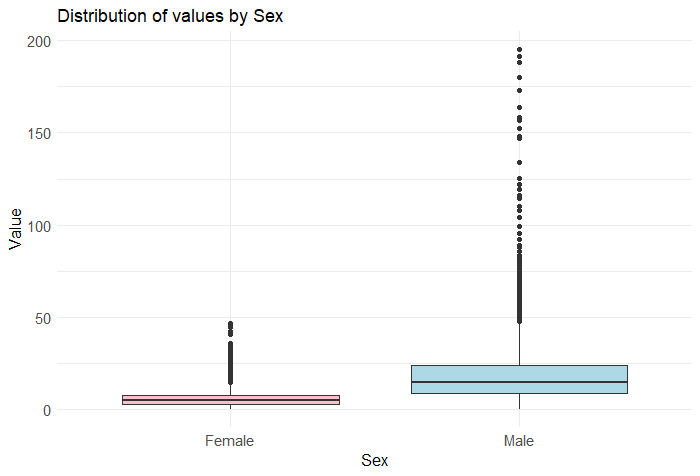
\includegraphics[width=.5\textwidth]{img/1 - Sex2.png}}
    \caption{Boxplot della distribuzione dei valori rispetto al sesso}
    \label{1sex}
\end{figure}
In questo modo è possibile apprezzare come esista una notevole differenza
nella distribuzione tra i sessi: è evidente che gli individui maschili compiono
con maggiore frequenza atti suicidari.

\begin{figure}[htbp]
    \centerline{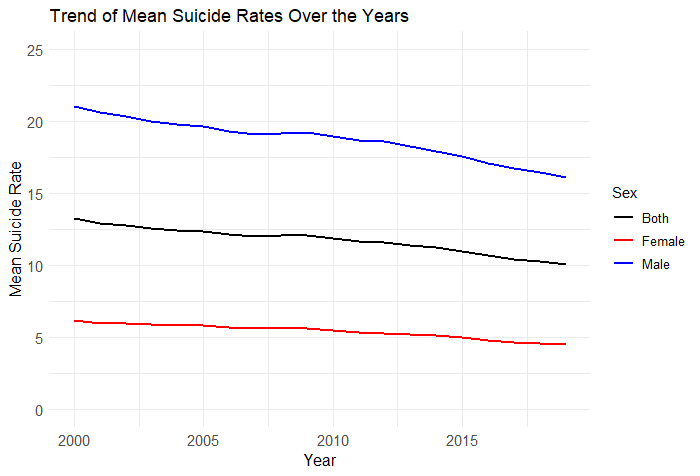
\includegraphics[width=.5\textwidth]{img/2 - Globtrend2.png}}
    \caption{Lineplot del trend dei suicidi medi globali ogni anno}
    \label{2globtrend}
\end{figure}
Ciò è constatabile anche osservando il trend globale del
tasso medio dei suicidi ogni anno riportato in Fig.~\ref{2globtrend}: il trend maschile
si attesta su valori significativamente più alti rispetto a quello femminile, mentre
il trend di Both esibisce un andamento intermedio tra i valori dei due sessi.

Si può inoltre osservare
che, nonostante il trend globale sia in declino, non c'è alcuna differenza
statisticamente significativa tra un anno e il successivo.
Possiamo apprezzare meglio questo andamento 
osservando la distribuzione dei valori anno per anno tramite il boxplot
in Fig.~\ref{3boxyears}.
\begin{figure}[htbp]
    \centerline{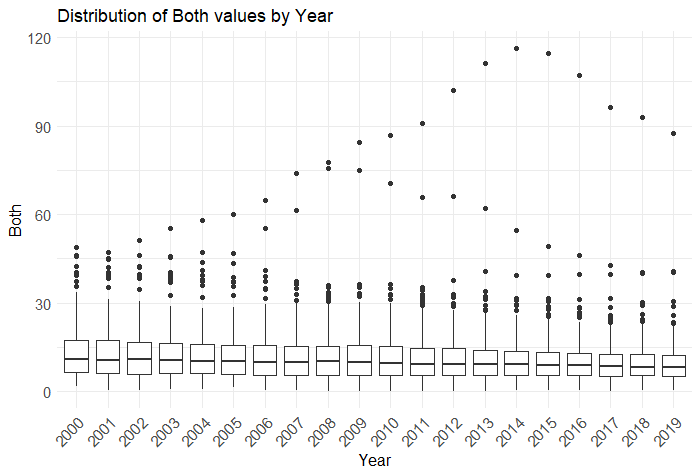
\includegraphics[width=.5\textwidth]{img/3 - Boxyears2.png}}
    \caption{Boxplot della distribuzione dei valori tra gli anni}
    \label{3boxyears}
\end{figure}
La differenza tra ciascun anno e il successivo è esigua ma ciononostante rilevabile: nel corso del ventennio
in esame, infatti, la distribuzione cambia notevolmente.
Andiamo infine ad analizzare il trend del tasso medio dei suicidi suddiviso
per regione del mondo secondo la ripartizione della WHO in Fig.~\ref{4wrtrend}.

\begin{figure}[htbp]
    \centerline{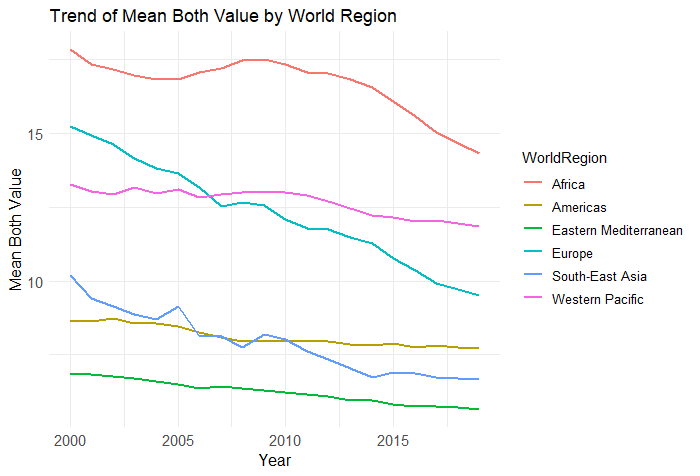
\includegraphics[width=.5\textwidth]{img/4 - WRTrend2.png}}
    \caption{Lineplot del trend dei suicidi medi ogni anno suddiviso per regione globale}
    \label{4wrtrend}
\end{figure}

In ogni regione è possibile osservare una comune tendenza negativa
del tasso dei suicidi, e la sostanziale consonanza degli andamenti statistici
è rilevabile anche nella sincrona presenza di eventi localizzati di crescita
(ad esempio nel 2008-2009) e decrescita.
A questo punto ci si potrebbe chiedere se alcuni gruppi
di paesi o persino le regioni globali presentino
distribuzioni annuali dei tassi di suicidi
senza differenze significative tra loro.
Al fine di articolare tale questione procederemo ora con l'analisi di
un primo gruppo di soggetti, formato dalle sei regioni globali e dalle loro medie annuali,
e poi di tre gruppi formati ognuno da sei paesi selezionati con diversi criteri.
Per semplificare l'analisi e ridurre il numero di rappresentazioni grafiche verranno presi in esame solo
gli anni dal 2014 al 2019.

\subsection{Primo gruppo - Regioni globali (WR)}
Utilizziamo il Box and Whisker Plot (BWPlot) in Fig.~\ref{5firstgroup} per visualizzare il
valor medio di Both in ogni regione del mondo, anno per anno.
\begin{figure}[htbp]
    \centerline{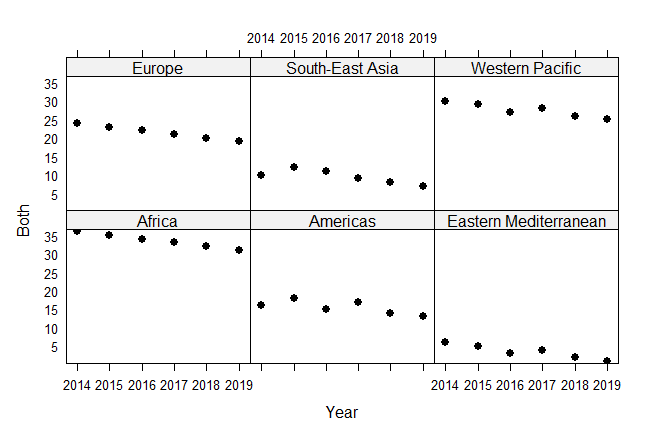
\includegraphics[width=.5\textwidth]{img/5 - Firstgroup.png}}
    \caption{BWPlot della media di Both anno per anno in ogni regione}
    \label{5firstgroup}
\end{figure}
Già dalla figura è possibile notare che, eccezione fatta per il declino generale
precedentemente discusso, non è rilevabile
alcun trend comune.
Tramite gli otto QQ-Plot in Fig.~\ref{6firstqq},
\begin{figure}[htbp]
    \centerline{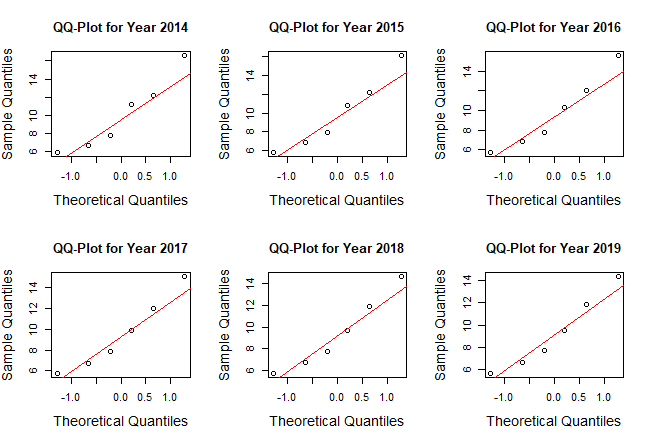
\includegraphics[width=.5\textwidth]{img/6 - Firstqq.png}}
    \caption{QQ-Plot dei valori medi di Both negli anni presi in esame}
    \label{6firstqq}
\end{figure}
uno per anno, si può osservare come sia
molto probabile che le medie dei dati raccolti ogni anno seguano una distribuzione normale.


\subsection{Secondo gruppo - Paese con PIL più alto per WR}

I paesi individuati come quelli con il PIL maggiore \cite{b6} all'interno della WR
d'appartenenza nel 2019 sono:
\begin{itemize}
    \item \textbf{United States of America} (USA) per Americas;
    \item \textbf{Germany} (DEU) per Europe;
    \item \textbf{China} (CHN) per Western Pacific;
    \item \textbf{Saudi Arabia} (SAU) per Eastern Mediterranean;
    \item \textbf{Nigeria} (NGA) per Africa;
    \item \textbf{India} (IND) per South-East Asia. 
\end{itemize}
Osserviamo dunque il BWPlot relativo in Fig.~\ref{7secondgroup}.
\begin{figure}[htbp]
    \centerline{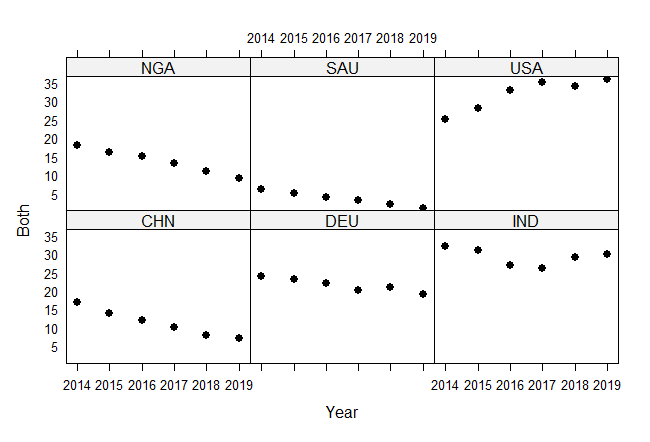
\includegraphics[width=.5\textwidth]{img/7 - Secondgroup.png}}
    \caption{BWPlot di Both anno per anno in ogni paese (2° gruppo)}
    \label{7secondgroup}
\end{figure}
\`E rilevabile un trend comune ad alcuni soggetti (ad es. NGA e CHN) mentre, prendendone
in considerazione altri (ad es. USA e IND) la consonanza è esigua.
In seguito verificheremo con un test opportuno se le distribuzioni differiscono significativamente
tra di loro o meno.
Tramite gli otto QQ-Plot in Fig.~\ref{8secondqq},
\begin{figure}[htbp]
    \centerline{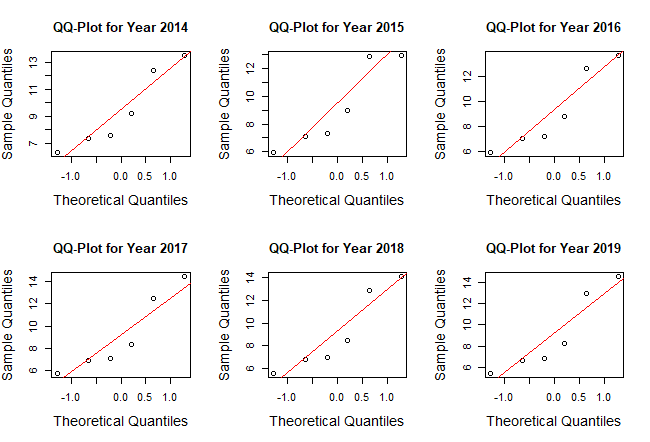
\includegraphics[width=.5\textwidth]{img/8 - Secondqq.png}}
    \caption{QQ-Plot dei valori Both negli anni presi in esame (2° gruppo)}
    \label{8secondqq}
\end{figure}
uno per anno, si può osservare come, anche in questo caso,
sia molto probabile che i dati raccolti annualmente seguano una distribuzione normale.



\subsection{Terzo gruppo - Paesi con tasso di suicidio più alto in assoluto}

I paesi individuati come quelli con il tasso di suicidio più alto
in assoluto sono:
\begin{itemize}
    \item \textbf{Lesotho} (LSO);
    \item \textbf{Guyana} (GUY);
    \item \textbf{Russian Federation} (RUS);
    \item \textbf{Eswatini} (SWZ);
    \item \textbf{Botswana} (BWA);
    \item \textbf{Kiribati} (KIR). 
\end{itemize}
Osserviamone il BWPlot in Fig.~\ref{9thridgroup}:
\begin{figure}[htbp]
    \centerline{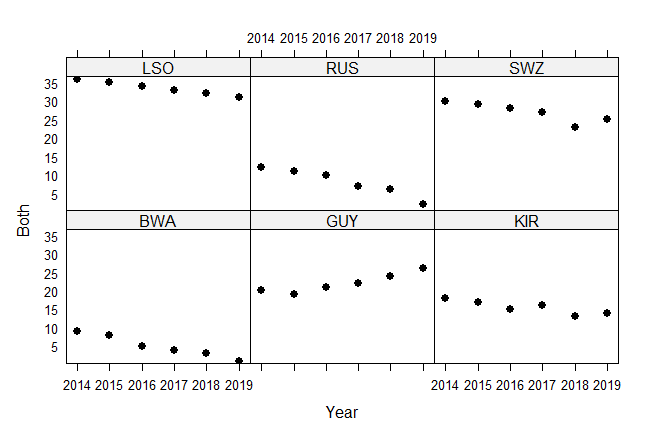
\includegraphics[width=.5\textwidth]{img/9 - Thirdgroup.png}}
    \caption{BWPlot di Both anno per anno in ogni paese (3° gruppo)}
    \label{9thridgroup}
\end{figure}
notiamo che un trend comune è difficile individuabile.
Riferendoci ai QQ-Plot in Fig.~\ref{10thirdqq} possiamo supporre che i dati non siano
distribuiti normalmente negli anni, andremo poi a verificare tale ipotesi nella sezione IV.
\begin{figure}[htbp]
    \centerline{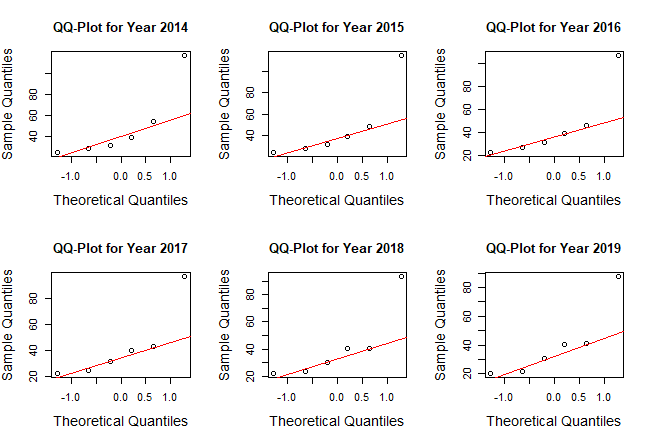
\includegraphics[width=.5\textwidth]{img/10 - Thirdqq.png}}
    \caption{QQ-Plot dei valori Both negli anni presi in esame (3° gruppo)}
    \label{10thirdqq}
\end{figure}

\subsection{Quarto gruppo - Paesi con tasso di suicidio più alto per WR}

I paesi on il tasso di suicidio più alto per la
WR d'appartenenza sono:
\begin{itemize}
    \item \textbf{Lesotho} (LSO) per Africa;
    \item \textbf{Guyana} (GUY) per Americas;
    \item \textbf{Russian Federation} (RUS) per Europe;
    \item \textbf{Somalia} (SOM) per Eastern Mediterranean;
    \item \textbf{Sri Lanka} (LKA) per South-East Asia;
    \item \textbf{Kiribati} (KIR) per Western Pacific. 
\end{itemize}
Relativamente a questi paesi osserviamo il BWPlot in Fig.~\ref{11fourthgroup}.
\begin{figure}[htbp]
    \centerline{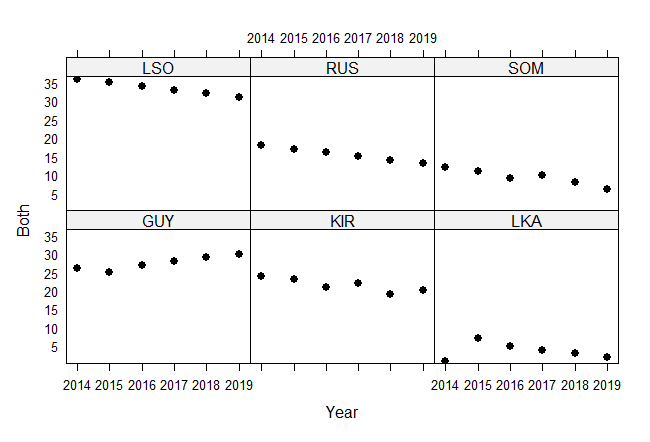
\includegraphics[width=.5\textwidth]{img/11 - Fourthgroup.png}}
    \caption{BWPlot di Both anno per anno in ogni paese (4° gruppo)}
    \label{11fourthgroup}
\end{figure}
Possiamo notare un trend comune.
Riferendoci ai QQ-Plot in Fig.~\ref{12fourthqq} possiamo supporre che i dati non siano
distribuiti normalmente negli anni, andremo poi a verificare tale ipotesi nella sezione IV.
\begin{figure}[htbp]
    \centerline{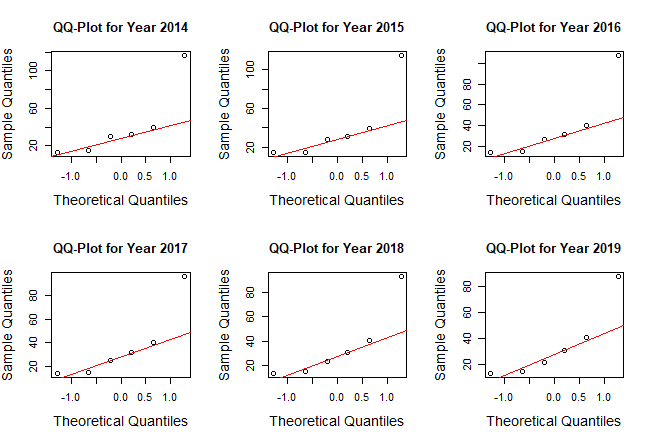
\includegraphics[width=.5\textwidth]{img/12 - Fourthqq.png}}
    \caption{QQ-Plot dei valori Both negli anni presi in esame (4° gruppo)}
    \label{12fourthqq}
\end{figure}

\section{Test statistici}

Si intende verificare che, all'interno dei gruppi selezionati,
i dati raccolti provengono ogni anno da distribuzioni che non differiscono
in maniera significativa tra di loro.
A tal fine, l'ANOVA a misure ripetute è il test più idoneo,
per il quale è tuttavia necessario andare a verificare la normalità,
l'omochedasticità e la sfericità delle misure.
Nell'eventualità in cui
anche una sola di queste assunzioni non venga rispettata occorre
ricorrere sul test non parametrico di Friedman.

\subsection{Verifica della normalità}

Le supposizioni sulla normalità dei dati vengono confermate
con il test di Shapiro-Wilk, i cui p-value vengono riportati nella Tab.~\ref{tab1}.
Solo i primi due gruppi presi in esame,
(gruppo delle medie delle WR e dei paesi con PIL più alto per WR)
infatti, rispettano il vincolo della normalità,
in quanto hanno tutti i p-value dei test relativi ai loro anni superiori a 0.05.
\begin{table}[htbp]
    \caption{Test di Shapiro-Wilk}
    \begin{center}
    \begin{tabular}{|c|c|c|c|c|c|c|}
    \hline
    \textbf{Gruppo}&\multicolumn{6}{|c|}{\textbf{Anni}} \\
    \cline{2-7} 
     & \textbf{2014} & \textbf{2015} & \textbf{2016} & \textbf{2017} & \textbf{2018} & \textbf{2019}\\
    \hline
    \textbf{Gruppo 1} & 0.531 & 0.672 & 0.690 & 0.705 & 0.708 & 0.719 \\\cline{1-7}
    \textbf{Gruppo 2} & 0.913 & 0.824 & 0.804 & 0.832 & 0.746 & 0.569 \\\cline{1-7}
    \textbf{Gruppo 3} & 0.018 & 0.011 & 0.017 & 0.026 & 0.021 & 0.056 \\\cline{1-7}
    \textbf{Gruppo 4} & 0.015 & 0.011 & 0.018 & 0.037 & 0.046 & 0.071 \\\cline{1-7}
    \hline
    \end{tabular}
    \label{tab1}
    \end{center}
\end{table}

\subsection{Verifica dell'omoschedasticità}

Poiché solo i primi due gruppi hanno dati distribuiti secondo una distribuzione normale
andremo ad utilizzare il test di Bartlett solo su questi due, i risultati,
riportati in Tab.~\ref{tab2}, mostrano come entrambi rispettino l'omoschedasticità.
\begin{table}[htbp]
    \caption{Test di Bartlett}
    \begin{center}
    \begin{tabular}{|c|c|c|}
    \hline
    \textbf{Gruppo} & \textbf{K-squared} & \textbf{p-value} \\
    \hline
    \textbf{Gruppo 1} & 0.27014 & 0.9982 \\\cline{1-3}
    \textbf{Gruppo 2} & 0.39744 & 0.9954 \\\cline{1-3}
    \hline
    \end{tabular}
    \label{tab2}
    \end{center}
\end{table}

\`E possibile fare un discorso analogo per gli ultimi due gruppi per cui è stato utilizzato il test di
Levene, più robusto rispetto a Bartlett nel caso di allontanamento dalla normalità.
Come si può notare in Tab.~\ref{tab3}, anche loro sono omoschedastici.
\begin{table}[htbp]
    \caption{Test di Levene}
    \begin{center}
    \begin{tabular}{|c|c|c|}
    \hline
    \textbf{Gruppo} & \textbf{F-value} & \textbf{p-value} \\
    \hline
    \textbf{Gruppo 3} & 0.037 & 0.9992 \\\cline{1-3}
    \textbf{Gruppo 4} & 0.016 & 0.9999 \\\cline{1-3}
    \hline
    \end{tabular}
    \label{tab3}
    \end{center}
\end{table}

\subsection{Verifica della sfericità}

Utilizzando la statistica di Greenhouse-Geisser notiamo come nessuno dei quattro gruppi
soddisfa la sfericità, in quanto i loro valori $\varepsilon$ riportati in Tab.~\ref{tab4},
si allontanano troppo da 1.
\begin{table}[htbp]
    \caption{Statistica di Greenhouse-Geisser}
    \begin{center}
    \begin{tabular}{|c|c|}
    \hline
    \textbf{Gruppo} & $\boldsymbol{\varepsilon}$\\
    \hline
    \textbf{Gruppo 1} & 0.2067 \\\cline{1-2}
    \textbf{Gruppo 2} & 0.2280 \\\cline{1-2}
    \textbf{Gruppo 3} & 0.2122 \\\cline{1-2}
    \textbf{Gruppo 4} & 0.2028 \\\cline{1-2}
    \hline
    \end{tabular}
    \label{tab4}
    \end{center}
\end{table}
Possiamo però valutare di utilizzare comunque ANOVA per i primi due gruppi
che soddisfano sia normalità che omoschedasticità, per
accertare se conferma il test di Friedman o meno (in ogni caso, sarà il test di Friedman
quello che considereremo significativo).

\subsection{Test di Friedman}

Per i vari gruppi riportiamo, nella Tab.~\ref{tab5}, i risultati del test di Friedman.
\begin{table}[htbp]
    \caption{Test di Friedman}
    \begin{center}
    \begin{tabular}{|c|c|c|}
    \hline
    \textbf{Gruppo} & $\boldsymbol{\chi}$\textbf{-squared} & \textbf{p-value} \\
    \hline
    \textbf{Gruppo 1} & 26.19 & 8.196$\times 10^{-5}$ \\\cline{1-3}
    \textbf{Gruppo 2} & 10.762 & 0.05631 \\\cline{1-3}
    \textbf{Gruppo 3} & 13.143 & 0.02208 \\\cline{1-3}
    \textbf{Gruppo 4} & 8.2857 & 0.1412 \\\cline{1-3}
    \hline
    \end{tabular}
    \label{tab5}
    \end{center}
\end{table}
Possiamo osservare come solo nel secondo e quarto gruppo 
(ovvero quello dei paesi con PIL più alto per WR e dei paesi con tasso di
suicidio più alto per WR)
il p-value supera 0.05
e possiamo dunque accettare l'ipotesi nulla, ovvero sia quella per cui non esistono differenze
statistiche significative all'interno di tali gruppi.
Ciò va a confermare quello che si poteva intuire dai BWPlot riportati per questi
due gruppi.
Nel primo gruppo, ovvero quello composto dalle sei WR e dai rispettivi tassi medi di suicidio per
anno, il p-value è estremamente basso, indice del fatto che,
contro l'ipotesi dell'assenza di differenze significative,
abbiamo una forte evidenza.
Effettuando su questo gruppo il
test di Wilcoxon coppia a coppia con la correzione di Benjamini-Hochberg,
i cui p-value sono riportati in Tab.~\ref{tab6}, possiamo osservare la presenza
di differenze significative in quasi ogni coppia di anni
messa a confronto.
\begin{table}[htbp]
    \caption{Test di Wilcoxon con correzione di Benjamini-Hochberg}
    \begin{center}
    \begin{tabular}{|c|c|c|c|c|c|}
    \hline
    \textbf{Anni} & \textbf{2014} & \textbf{2015} & \textbf{2016} & \textbf{2017} & \textbf{2018} \\
    \hline
    \textbf{2015} & 0.438 & - & - & - & - \\ \hline
    \textbf{2016} & 0.108 & 0.043 & - & - & - \\ \hline
    \textbf{2017} & 0.078 & 0.043 & 0.438 & - & - \\ \hline
    \textbf{2018} & 0.043 & 0.043 & 0.043 & 0.043 & - \\ \hline
    \textbf{2019} & 0.043 & 0.043 & 0.043 & 0.043 & 0.043 \\ 
    \hline
    \end{tabular}
    \label{tab6}
    \end{center}
\end{table}

\subsection{ANOVA a misure ripetute}

Il primo e il secondo gruppo non rispettano le supposizioni per l'ANOVA a misure ripetute
unicamente perché si allontanano dalla sfericità.
Visti i risultati del test di Friedman, controlliamo se l'ANOVA a misure ripetute li conferma
o meno.
In Tab.~\ref{tab7} 
\begin{table}[htbp]
    \caption{ANOVA a misure ripetute}
    \begin{center}
    \begin{tabular}{|c|c|c|}
    \hline
    \textbf{Gruppo} & \textbf{F-value} & \textbf{p-value} \\
    \hline
    \textbf{Gruppo 1} & 4.482 & 0.0878 \\\cline{1-3}
    \textbf{Gruppo 2} & 0.229 & 0.652 \\\cline{1-3}
    \hline
    \end{tabular}
    \label{tab7}
    \end{center}
\end{table}
si riporta che, per entrambi i gruppi, l'ANOVA ci restituisce un p-value superiore allo 0.05.
Nel secondo gruppo, in cui accettiamo l'ipotesi nulla anche con il test di Friedman,
otteniamo persino 0.652.
Il primo gruppo si attesta sopra la soglia con 0.0878, utilizzando ANOVA accettiamo quindi
l'ipotesi nulla per la quale, riferendoci invece a Friedman, vi erano fortissime evidenze contrarie.
Considerando però la sfericità non rispettata, i risultati ottenuti con l'ANOVA sono molto
meno significativi.


\section{Conclusioni}

Nell'analisi appena presentata è possibile osservare come, in determinati periodi di tempo
e in determinati gruppi, nello specifico quello dei paesi con PIL più alto per WR e
quello dei paesi con tasso di suicidio più alto per WR, non esistono differenze
significative nella distribuzione annuale del tasso dei suicidi.
Tuttavia, anche solo prendendo in esame due gruppi statistici che condividono quattro paesi
di riferimento e differiscono per due, otteniamo risultati completamente differenti
(come rilevato con il terzo e il quarto gruppo).
Considerando la particolarità del fenomeno, la cui causa può essere individuata nelle motivazioni più disparate,
la presente analisi si propone come base per studi futuri, i quali potrebbero
unire il dataset in esame
con altri atti a descrivere fattori sociali, economici o geopolitici potenzialmente
influenti sulla distribuzione del tasso dei suicidi.


\begin{thebibliography}{00}
    \bibitem{b1} Shneidman ES. ``The definition of suicide''. New York, NY and London: John Wiley and sons; 1985.
    \bibitem{b2} Gvion Y, Apter A. ``Suicide and suicidal behavior''. Public Health Reviews. 2012;34: epub ahead of print.
    \bibitem{b3} Värnik, P. ``Suicide in the world''. Int. J. Environ. Res. Public Health 2012, 9, 760-771. https://doi.org/10.3390/ijerph9030760 
    \bibitem{b4} World Health Organization. (2023). ``Suicide rates''. Recuperato da https://www.who.int/data/gho/data/themes/mental-health/suicide-rates
    \bibitem{b5} Statistics Canada. (2023). ``Age-standardized rates''. Recuperato da https://www.statcan.gc.ca/en/dai/btd/asr
    \bibitem{b6} countryeconomy.com. (2023). ``GDP - Gross Domestic Product 2019''. Recuperato da https://countryeconomy.com/gdp?year=2019
\end{thebibliography}

\end{document}
